\documentclass[a4paper]{article}
\usepackage[left=80pt,right=80pt,top=60pt,bottom=60pt]{geometry}
\usepackage[font=small,labelfont=bf]{caption}
\usepackage{float}
\usepackage{graphicx}
\usepackage{amssymb}
\usepackage{amsmath}
\usepackage{array}
\usepackage{hyperref}
\usepackage{multirow}

\setlength\parindent{0pt}
\graphicspath{ {./imgs/} }

\title {
    Object Oriented Analysis and Design \\
    Course project - Application and Recruitment Environment
}


\author{
    Instructor: Assoc. Prof. Dr. Truong Ninh Thuan
    \\\\
    Students:\\
    \begin{tabular}{ l l }
        Vu Ngoc Hien & 19021268 \\ 
        Le Truong Giang & 19021260 \\
        Nguyen Vinh Quang & 1902????
    \end{tabular}
}

\begin{document}
\maketitle
\pagebreak

\tableofcontents
\pagebreak

\listoffigures
\pagebreak

\section{Requirements}
    \subsection{Problem statement}
        \subsubsection{Problem}
        something about this shit?
        
        \subsubsection{Solution}
        something about this shit?
        
    \subsection{Glossary}
    something huh
    
    \subsection{Supplementary specifications}
    something huh

    \subsection{Use-case model}

    \begin{figure}[H]
        \centering
        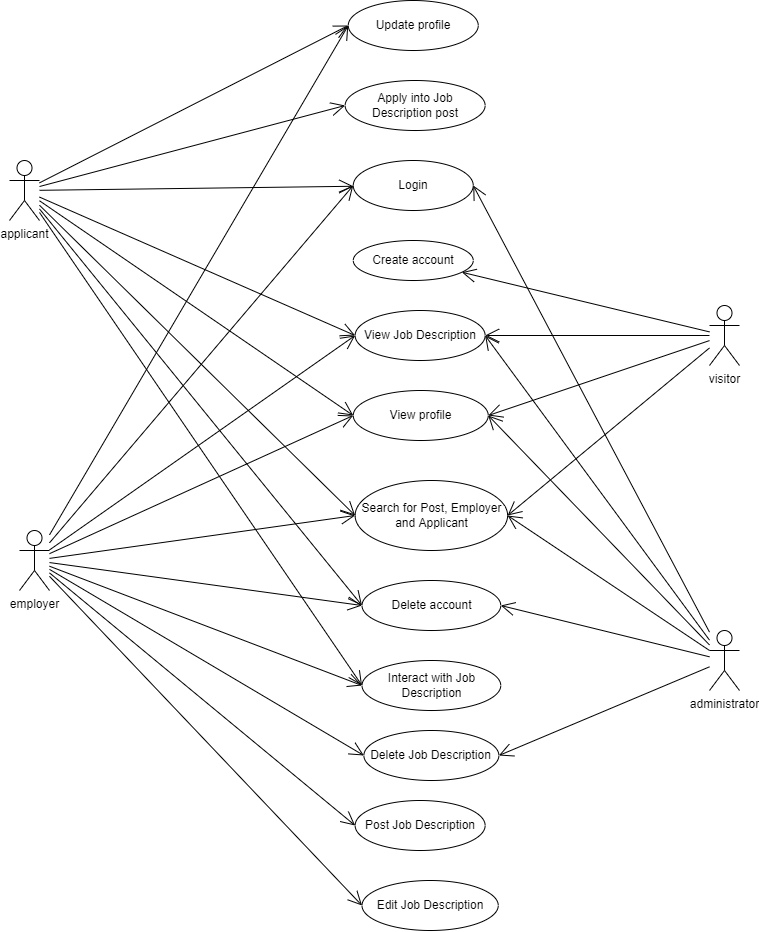
\includegraphics[width=0.8\textwidth]{usecase_model.drawio.png}
        \caption{Use-case model}
        \label{fig:fig1}
    \end{figure}

        \subsubsection{View profile}
        \textbf{Description:}
        \begin{itemize}
            \item As a visitor or logged in user, views the profile information of other users on the system.
            \item Depending on the permission level, the information that are made available is different.
        \end{itemize}

        \textbf{Actors:}
        \begin{itemize}
            \item Visitor.
            \item Applicant.
            \item Employer.
            \item Administrator.
            \item User database.
        \end{itemize}

        \textbf{Trigger:}
        \begin{itemize}
            \item Users clicking on another user's name or profile picture within the website.
            \item Users visiting the direct link to another user's profile page.
            \item Logged in users clicking on their own profile picture.
        \end{itemize}

        \textbf{Preconditions:}
        \begin{itemize}
            \item The user exists in the user database with their basic information
            \item The user's account is not locked.
        \end{itemize}

        \textbf{Postconditions:}
        \begin{itemize}
            \item The user is presented with the profile.
            \item Sections and options are provided based on authentication status, permissions and available information.
            \item The visit gets logged if the profile owner chose to do so (for statistical reasons).
        \end{itemize}

        \textbf{Flow of events:}
        \begin{itemize}
            \item User click on another user's feature (e.g., name, avatar) within the site (in post, feeds, suggestions).
            \item The system determines what data get shown and what get hidden based on the permission level and authentication status.
            \item The information is displayed.
        \end{itemize}

        \textbf{Alternative flows:}
        \begin{itemize}
            \item Flow 1:
            \begin{itemize}
                \item The user clicks on their own profile.
                \item The page is displayed with all available information with ability to edit the information stored.
            \end{itemize}
            \item Flow 2:
            \begin{itemize}
                \item The user clicks a link from a different website linking to the user profile.
                \item The system determines what data get shown and what get hidden based on the permission level and authentication status.
                \item The information is displayed.
            \end{itemize}
        \end{itemize}

        \textbf{Exception flows:}
        \begin{itemize}
            \item Flow 1:
            \begin{itemize}
                \item The owner blocked public visitors from seeing their profile.
                \item The site displays an error message.
            \end{itemize}
            \item Flow 2:
            \begin{itemize}
                \item User clicking a link.
                \item The user does not exist in the database.
                \item The site displays an error message.
            \end{itemize}
        \end{itemize}

        \subsubsection{Create Account}
        \textbf{Description:}
        \begin{itemize}
            \item As a visitor, create an account on the system in order to access its personalized features, or features that requires identity confirmation.
        \end{itemize}

        \textbf{Actor:}
        \begin{itemize}
            \item Visitor.
            \item Authentication backends.
        \end{itemize}

        \textbf{Trigger:}
        \begin{itemize}
            \item User wanting to logs into the system when they don't have an existing account.
        \end{itemize}

        \textbf{Precondition:}
        \begin{itemize}
            \item User does not have an account.
            \item User has internet connection.
        \end{itemize}

        \textbf{Postcondition:}
        \begin{itemize}
            \item User gets logged into the application.
            \item Basic user authentication information is written into the database.
        \end{itemize}

        \textbf{Flow of events:}
        \begin{itemize}
            \item User accesses the website
            \item User intentionally opt to register / User attempts to access a website part that requires authentication
            \item User inputs basic information such as their email address, name and password of choice
            \item Authentication systems sent an email to the chosen inbox.
            \item User verifies by opening their email inbox and click the link
            \item The system saves the user's sign in information and ask for extra information as needed
        \end{itemize}

        \textbf{Alternative flows:}
        None.

        \textbf{Exceptions:}
        \begin{itemize}
            \item User does not have internet connection.
            \begin{itemize}
                \item User cannot register.
            \end{itemize}
            \item User already have an account associated with an email.
            \begin{itemize}
                \item Notifies user and offer to reset password.
            \end{itemize}
            \item User fails to confirm their password.
            \item User's email is blocked from registering.
        \end{itemize}
        
        \textbf{Business rules:}
        \begin{itemize}
            \item Deny account registration if there are more than three registration attempts from the same computer within the span of a day (24 hours).
        \end{itemize}

        \textbf{Non-functional requirements:}
        \begin{itemize}
            \item User passwords are hashed with a salt for security.
        \end{itemize}

        \subsubsection{Login}
        \textbf{Description:}
        \begin{itemize}
            \item As an existing user (applicant, employer or admin), login to an existing account.
        \end{itemize}

        \textbf{Actor:}
        \begin{itemize}
            \item Applicant.
            \item Employer.
            \item Admin.
            \item Authentication backends.
        \end{itemize}

        \textbf{Trigger:}
        \begin{itemize}
            \item User choosing to login on the interface
            \item User visiting contents that requires authentication
        \end{itemize}

        \textbf{Precondition:}
        \begin{itemize}
            \item User already have an account in the authentication database.
            \item User account have proper permissions to login.
            \item User has internet connection.
        \end{itemize}

        \textbf{Postcondition:}
        \begin{itemize}
            \item User gets logged in to the account.
            \item The activity is logged into the user's Activity Log.
        \end{itemize}

        \textbf{Flow of events:}
        \begin{itemize}
            \item User choose to login from the user interface or access a page that requires authentication.
            \item The system checks for any existing session token on the device.
            \item The user provides their email address and password of their choosing.
            \item The system compares the information the user provides with what is stored in the authentication database.
            \item The system logs the user in and set a session token on the device.
        \end{itemize}
        
        \textbf{Alternative flows:}
        None.

        \textbf{Exceptions flow:}
        \begin{itemize}
            \item If the system found an existing session token on the device, instead of prompting the user for the account info, logs the user in if the token is valid.
            \item If the user-provided information is not correct, prompt the user and offer password reset.
            \item If the account is blocked from login, notifies the user and sign out automatically.
            \item If the user does not have internet connection before the data is sent to the server, the system will cache the data.
        \end{itemize}

        \subsubsection{Update profile}
        \textbf{Description:}
        \begin{itemize}
            \item User go to profile page and update information. New information will be saved and displayed on profile page after user click update button.
            \item This feature apply to both employer and applicant.
        \end{itemize}

        \textbf{Actor:}
        \begin{itemize}
            \item Applicant or employer.
        \end{itemize}

        \textbf{Trigger:}
        \begin{itemize}
            \item User wanting to update profile information.
        \end{itemize}

        \textbf{Precondition:}
        \begin{itemize}
            \item User has an account (not administrator account).
            \item User logged in.
            \item User has internet connection.
        \end{itemize}

        \textbf{Postcondition:}
        \begin{itemize}
            \item User profile information is updated.
        \end{itemize}

        \textbf{Flow of events:}
        \begin{itemize}
            \item User go to profile page.
            \item User update new information. User can add new section information (e.g. education, experience, etc.) or update existing information.
            \item User click update button.
            \item System save new information.
            \item System display new information on profile page.
        \end{itemize}

        \textbf{Alternative flow:}
        \begin{itemize}
            \item User click cancel button.
            \item System display old information on profile page.
        \end{itemize}

        \textbf{Exception flow:}
        \begin{itemize}
            \item User has no internet connection.
            \item System display error message.
        \end{itemize}

        \textbf{Business rules:}
        \begin{itemize}
            \item User can only update information of his/her own profile.
        \end{itemize}

        \textbf{Non-functional requirements:}
        None

        \subsubsection{Apply into job description post}
        \textbf{Description:}
        \begin{itemize}
            \item User go to job description post page and apply for the job. User can apply for multiple jobs.
            \item This feature apply to applicant only.
        \end{itemize}

        \textbf{Actor:}
        \begin{itemize}
            \item Applicant.
            \item Backend system.
        \end{itemize}

        \textbf{Trigger:}
        \begin{itemize}
            \item User wanting to apply for a job in a job description post.
        \end{itemize}

        \textbf{Precondition:}
        \begin{itemize}
            \item User has an applicant account.
            \item User logged in.
            \item User has internet connection.
        \end{itemize}

        \textbf{Postcondition:}
        \begin{itemize}
            \item User apply for a job in a job description post.
        \end{itemize}

        \textbf{Flow of events:}
        \begin{itemize}
            \item User go to job description post page.
            \item User click apply button.
            \item System shows a textbox for user to write a cover letter or simply a message/comment (optional).
            \item System save user's application.
            \item System send notification to employer and applicant to confirm.
        \end{itemize}

        \textbf{Alternative flow:}
        \begin{itemize}
            \item User click cancel button.
            \item System display job description post page.
        \end{itemize}

        \textbf{Exception flow:}
        \begin{itemize}
            \item User has no internet connection.
            \item System display error message.
        \end{itemize}

        \textbf{Business rules:}
        \begin{itemize}
            \item Each user can apply for only onetime in a job description post.
        \end{itemize}

        \textbf{Non-functional requirements:}
        None

        \subsubsection{Interact with job description}
        \textbf{Description:}
        \begin{itemize}
            \item User go to job description post page and interact with the job description post. User can like, dislike, comment the job description post.
            \item This feature apply to both applicant and employer.
        \end{itemize}

        \textbf{Actor:}
        \begin{itemize}
            \item Applicant or employer.
            \item Backend system.
        \end{itemize}

        \textbf{Trigger:}
        \begin{itemize}
            \item User wanting to interact with a job description post.
        \end{itemize}

        \textbf{Precondition:}
        \begin{itemize}
            \item User has an account (not administrator account).
            \item User logged in.
            \item User has internet connection.
        \end{itemize}

        \textbf{Postcondition:}
        \begin{itemize}
            \item User's interaction with a job description post is saved and displayed.
        \end{itemize}

        \textbf{Flow of events:}
        \begin{itemize}
            \item User go to job description post page.
            \item User click like, dislike button or leave a comment.
            \item System save user's interaction.
            \item System display user's interaction on job description post page.
        \end{itemize}

        \textbf{Alternative flow:}
        \begin{itemize}
            \item User stop commenting on job description post.
            \item System display job description post page.
        \end{itemize}

        \textbf{Exception flow:}
        \begin{itemize}
            \item User has no internet connection.
            \item System display error message.
        \end{itemize}

        \textbf{Business rules:}
        \begin{itemize}
            \item User can only have one like or dislike on a job description post.
            \item User can leave multiple comments on a job description post.
        \end{itemize}

        \textbf{Non-functional requirements:}
        None

        \subsubsection{Post job description}
        \textbf{Description:}
        \begin{itemize}
            \item Employer click create recruitment announcement and post a job description. Employer can post multiple job descriptions.
            \item This feature apply to employer only.
        \end{itemize}

        \textbf{Actor:}
        \begin{itemize}
            \item Employer.
            \item Backend service and database.
        \end{itemize}

        \textbf{Trigger:}
        \begin{itemize}
            \item Employer wanting to post a job description for recruitment.
        \end{itemize}

        \textbf{Precondition:}
        \begin{itemize}
            \item Employer has an employer account.
            \item Employer logged in.
            \item Employer has internet connection.
        \end{itemize}

        \textbf{Postcondition:}
        \begin{itemize}
            \item Employer post a job description for recruitment.
        \end{itemize}

        \textbf{Flow of events:}
        \begin{itemize}
            \item Employer click create recruitment announcement button.
            \item Employer fill in job description information.
            \item Employer click post button.
            \item System save job description information.
            \item System display job description post page.
        \end{itemize}

        \textbf{Alternative flow:}
        \begin{itemize}
            \item Employer stop editing job description information and close browser/tab or direct to another site or press cancel button.
            \item System display a warning message to ask employer weather to save a draft or not.
            \item Employer choose to save a draft or not. If yes, system save job description information as a draft in user's local storage. If no, system discard job description information.
        \end{itemize}

        \textbf{Exception flow:}
        \begin{itemize}
            \item Employer has no internet connection.
            \item System auto save job description information as a draft in employer's profile page by caching the draft in employer's device.
            \item System display error message.
        \end{itemize}

        \textbf{Business rules:}
        \begin{itemize}
            \item Employer can only post one job description in a recruitment announcement.
            \item Employer can post multiple job descriptions in multiple recruitment announcements.
        \end{itemize}

        \subsubsection{View job description post}
        \textbf{Description:}
        \begin{itemize}
            \item User go to job description post page and view the job description post.
        \end{itemize}

        \textbf{Actor:}
        \begin{itemize}
            \item Applicant.
            \item Employer.
            \item Administrator.
            \item Visitor.
            \item Backend service and database.
        \end{itemize}

        \textbf{Trigger:}
        \begin{itemize}
            \item User wanting to view a job description post.
            \item User search for a specific job description post.
        \end{itemize}

        \textbf{Precondition:}
        \begin{itemize}
            \item User has internet connection.
            \item Database service is available.
        \end{itemize}

        \textbf{Postcondition:}
        \begin{itemize}
            \item Job description post is displayed.
        \end{itemize}

        \textbf{Flow of events:}
        \begin{itemize}
            \item User goes to the website.
            \item User type a keyword related to the job in the search box.
            \item The website displays several job descriptions posts.
            \item User selects a job description post.
            \item The website displays the full job description post.
        \end{itemize}

        \textbf{Alternative flow:}
        \begin{itemize}
            \item Flow 1:
            \begin{itemize}
                \item User goes to the website.
                \item User type a keyword related to the job in the search box.
                \item The website displays several job descriptions posts.
                \item User selects a job description post.
                \item The website displays the full job description post.
            \end{itemize}
            \item Flow 2:
            \begin{itemize}
                \item User click on a link to a job description post.
                \item The website displays the full job description post.
            \end{itemize}
        \end{itemize}

        \textbf{Exception flow:}
        \begin{itemize}
            \item Flow 1:
            \begin{itemize}
                \item User cannot find any job description posts.
                \item Display a notification message.
            \end{itemize}
            \item Flow 2:
            \begin{itemize}
                \item User accesses a deleted job description post.
                \item Display an error message.
            \end{itemize}
        \end{itemize}

        \textbf{Business rules:}
        \begin{itemize}
            \item User cannot access a deleted job description post.
        \end{itemize}

        \subsubsection{Edit Job description post}
        \textbf{Description:}
        \begin{itemize}
            \item Employer wants to change the content of a job description post.
        \end{itemize}

        \textbf{Actor:}
        \begin{itemize}
            \item Employer.
            \item Backend service and database.
        \end{itemize}

        \textbf{Trigger:}
        \begin{itemize}
            \item Employer wants to change the content of a job description post.
        \end{itemize}

        \textbf{Precondition:}
        \begin{itemize}
            \item Employer has an employer account.
            \item Employer logged in.
            \item Employer has internet connection.
            \item Employer is viewing his/her job description post.
        \end{itemize}

        \textbf{Postcondition:}
        \begin{itemize}
            \item Employer has changed the content of a job description post.
        \end{itemize}

        \textbf{Flow of events:}
        \begin{itemize}
            \item User accesses the website.
            \item User selects a job description post.
            \item User click edit button.
            \item User modifies the content of the job description post.
            \item User saves the changes.
            \item The change has updated on the system.
            \item System display job description post page.
        \end{itemize}

        \textbf{Alternative flow:}
        \begin{itemize}
            \item User accesses the website.
            \item User selects a job description post.
            \item User click edit button.
            \item User modifies the content of the job description post.
            \item User close browser/tab or direct to another site or press cancel button.
            \item System display a warning message to ask user if the user wants to keep editing. If yes, the browser cancel closing/redirect keep editing. If no, system discard the changes.
        \end{itemize}

        \textbf{Exception flow:}
        \begin{itemize}
            \item User attempt to open more than 1 editor for 1 post at a time point.
            \item Display an error message.
        \end{itemize}

        \textbf{Business rules:}
        \begin{itemize}
            \item User can only open an editor for one post at a time point.
            \item User cannot edit other employer's job description posts.
        \end{itemize}

        \subsubsection{Delete Job description post}
        \textbf{Description:}
        \begin{itemize}
            \item User, as an employer, delete a job description posts.
            \item User, as an administrator, delete a post that is considered not a job description.
        \end{itemize}

        \textbf{Actor:}
        \begin{itemize}
            \item Employer.
            \item Administrator.
            \item Backend service and database.
        \end{itemize}

        \textbf{Trigger:}
        \begin{itemize}
            \item A job description post has expired or no longer needed.
        \end{itemize}

        \textbf{Precondition:}
        \begin{itemize}
            \item User has an internet connection.
            \item User has an employer/administration account.
            \item User logged in.
            \item The employer owned the job description post (this is not required for administration).
        \end{itemize}

        \textbf{Postcondition:}
        \begin{itemize}
            \item A job description post is removed from the database.
        \end{itemize}
        
        \textbf{Flow of events:}
        \begin{itemize}
            \item User accesses the website.
            \item User selects a description post or view a description post.
            \item User selects the remove option.
            \item The system ask for confirmation.
            \item The description post is removed from the database.
        \end{itemize}

        \textbf{Exception flow:}
        \begin{itemize}
            \item User attempt to delete a deleted job description post.
            \item Display an error message.
        \end{itemize}

        \textbf{Business rules:}
        \begin{itemize}
            \item User can use only one delete request on one job description post.
            \item User cannot delete other employer's job description post (except administrator).
        \end{itemize}

        \subsubsection{Delete Account}
        \textbf{Description:}
        \begin{itemize}
            \item The user can delete their account along with their associated data from the respective databases of the site.
            \item An administrator can delete a user's account upon their request or due to site rules violations.
        \end{itemize}

        \textbf{Actor:}
        \begin{itemize}
            \item Employer.
            \item Applicant.
            \item Administrator.
            \item Backend authentication.
        \end{itemize}
        
        \textbf{Trigger:}
        \begin{itemize}
            \item The user selecting the option to delete their account.
            \item An admin deleting an account from administration tools.
        \end{itemize}

        \textbf{Precondition:}
        \begin{itemize}
            \item The user is logged in and able to access their account settings.
            \item An administrator is authorized to manage user accounts.
            \item Employer or Applicant has internet connection.
        \end{itemize}

        \textbf{Postcondition:}
        \begin{itemize}
            \item The user login info and user data are deleted from all systems.
            \item The user may or may not re-register an account with the same email.
        \end{itemize}

        \textbf{Flow of events:}
        \begin{itemize}
            \item The user logs into their account.
            \item The user opens the account settings.
            \item The user chooses to delete their account.
            \item The user confirms with their password.
            \item The system verifies the password and ask for confirmation.
            \item The system deletes the user's data and authorization information.
        \end{itemize}

        \textbf{Alternative flow:}
        \begin{itemize}
            \item An admin logs into his/her account.
            \item The admin selects a user account and choose the option to delete it.
            \item The system asks if the user should be able to recreate an account with the same email.
            \item The system asks for confirmation.
            \item The system logs the deletion in the Audit log and sets a flag if the user is denied from re-registering.
        \end{itemize}

        \textbf{Exception flow:}
        \begin{itemize}
            \item Flow 1:
            \begin{itemize}
                \item The user has no internet connection.
                \item The system displays an error message.
            \end{itemize}
            \item Flow 2:
            \begin{itemize}
                \item The user fails to verify their password upon deletion.
            \end{itemize}
        \end{itemize}

        \subsubsection{Searching tool}
        \textbf{Description:}
        \begin{itemize}
            \item User search information from the website about job descriptions, employers, and applicants.
        \end{itemize}

        \textbf{Actor:}
        \begin{itemize}
            \item Applicant.
            \item Employer.
            \item Administrator.
            \item Visitor.
            \item Backend search engine.
        \end{itemize}

        \textbf{Trigger:}
        \begin{itemize}
            \item User wants to search for information about a typical job, an employer, or an applicant.
        \end{itemize}

        \textbf{Precondition:}
        \begin{itemize}
            \item User has internet connection.
        \end{itemize}

        \textbf{Postcondition:}
        \begin{itemize}
            \item The website displays several results about the information user is looking for.
        \end{itemize}
        
        \textbf{Flow of events:}
        \begin{itemize}
            \item User accesses the website.
            \item User clicks the search bar and type keywords in the search box.
            \item The website displays several results about the information user is looking for.
        \end{itemize}

        \textbf{Alternative flow:}
        \begin{itemize}
            \item User click on a link to a search result.
            \item The website displays several results about the information user is looking for.
        \end{itemize}

        \textbf{Exception flow:}
        \begin{itemize}
            \item The search engine does not find any information.
            \item The system displays a message not finding any job description post or employer or applicant.
        \end{itemize}

        \textbf{Business rules:}
        \begin{itemize}
            \item The search engine will search for information in the database.
            \item The search engine will search for information in the job description post, employer, and applicant.
        \end{itemize}
\section{Use-case realisations}
    \subsection{Sequence diagrams}

    \begin{figure}[H]
        \centering
        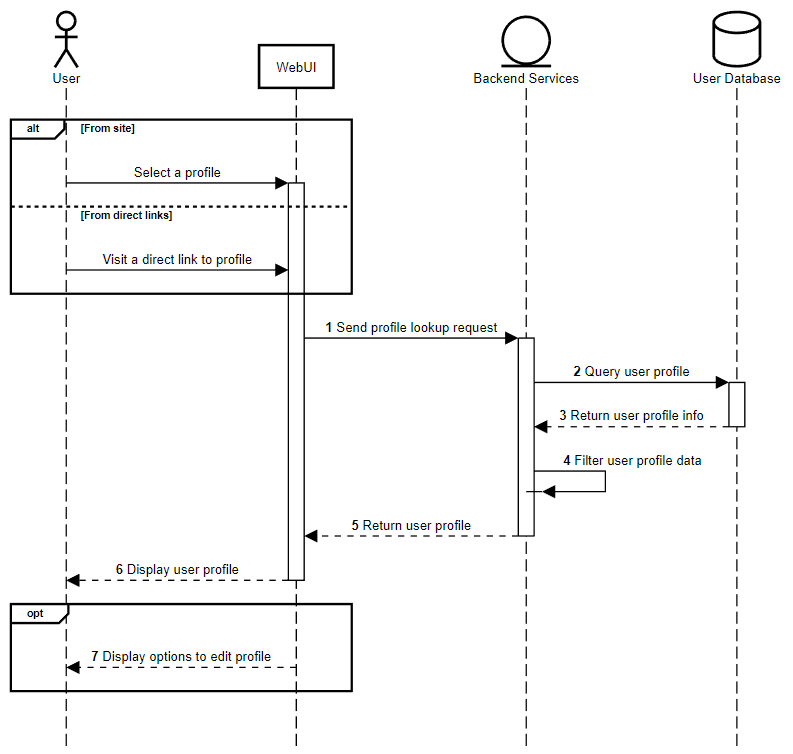
\includegraphics[width=1.0\textwidth]{view_profile.png}
        \caption{Sequence diagram for the use profile use case (basic flow)}
        \label{fig:fig2}
    \end{figure}

    \begin{figure}[H]
        \centering
        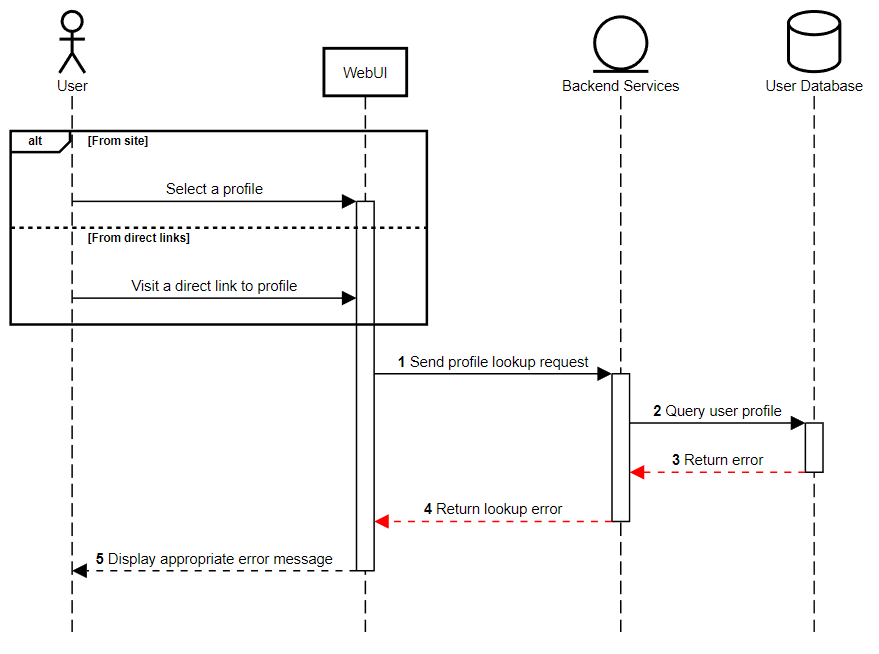
\includegraphics[width=1.0\textwidth]{view_profile (exception).png}
        \caption{Sequence diagram for the use profile use case (exception flow)}
        \label{fig:fig3}
    \end{figure}

    \begin{figure}[H]
        \centering
        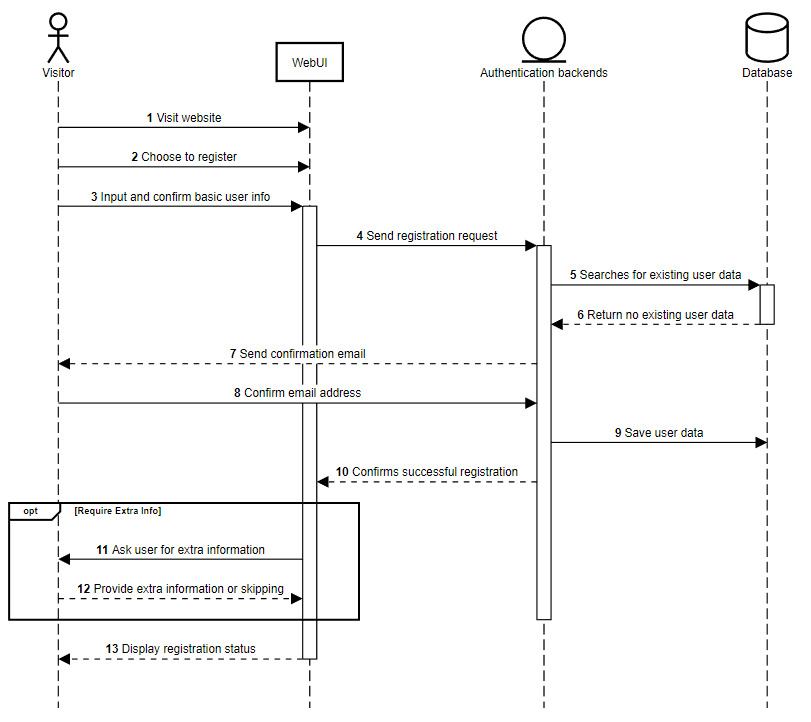
\includegraphics[width=1.0\textwidth]{create_account.png}
        \caption{Sequence diagram for the create account use case (basic flow)}
        \label{fig:fig4}
    \end{figure}

    \begin{figure}[H]
        \centering
        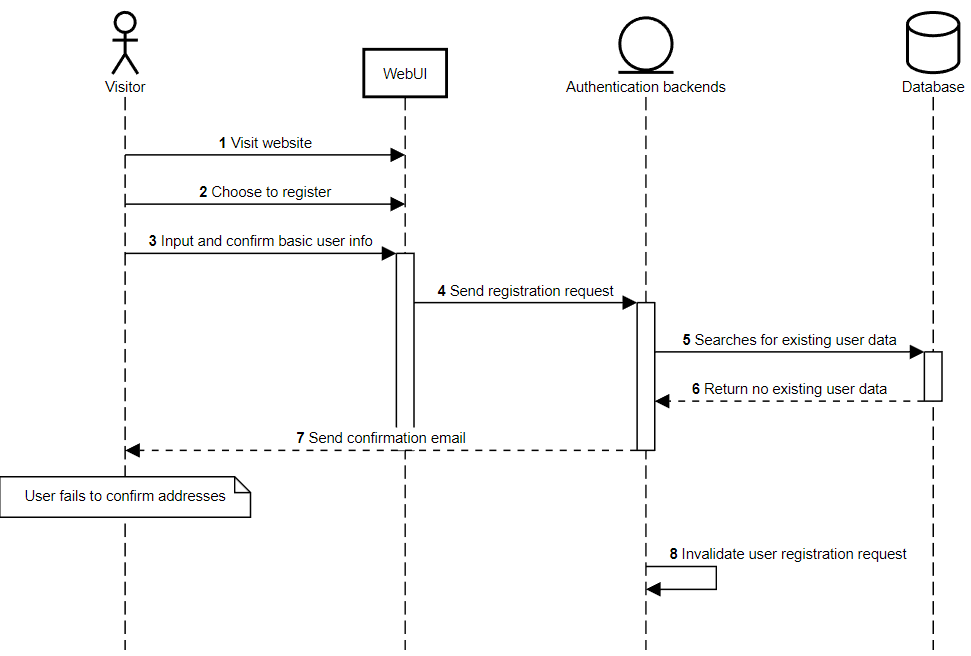
\includegraphics[width=1.0\textwidth]{create_account (unconfirmed email).png}
        \caption{Sequence diagram for the create account use case (unconfirmed email exception)}
        \label{fig:fig5}
    \end{figure}

    \begin{figure}[H]
        \centering
        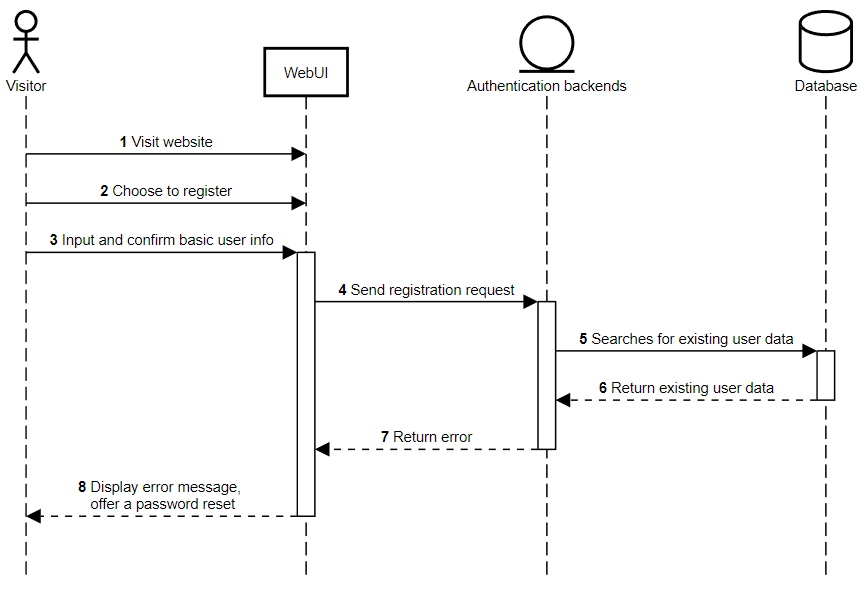
\includegraphics[width=1.0\textwidth]{create_account_(user exist).png}
        \caption{Sequence diagram for the create account use case (user exist exception)}
        \label{fig:fig6}
    \end{figure}

    \begin{figure}[H]
        \centering
        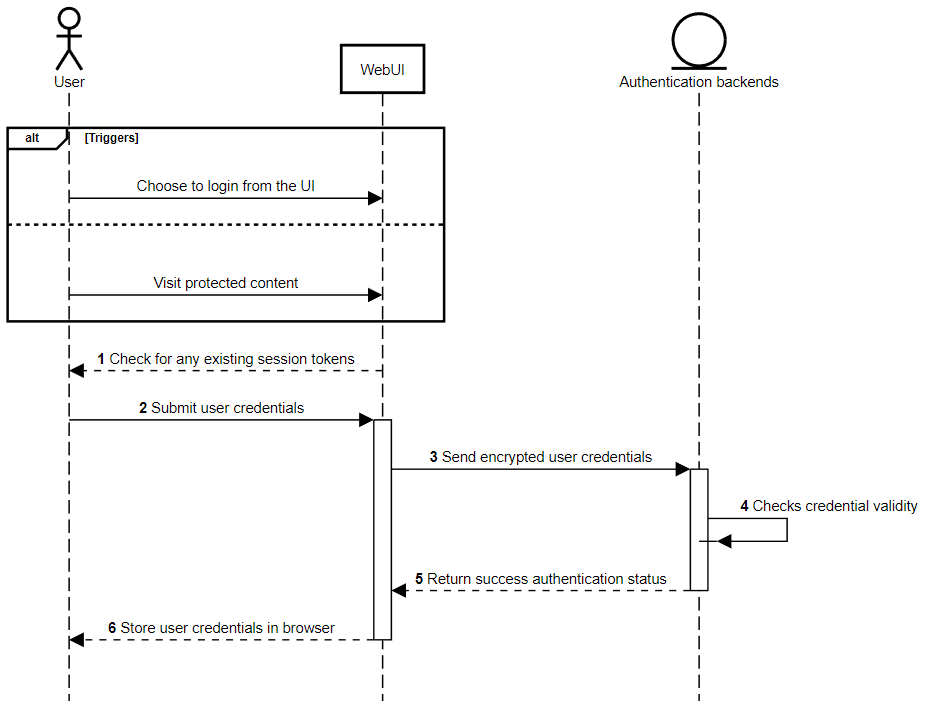
\includegraphics[width=1.0\textwidth]{login.png}
        \caption{Sequence diagram for the login use case (basic flow)}
        \label{fig:fig7}
    \end{figure}

    \begin{figure}[H]
        \centering
        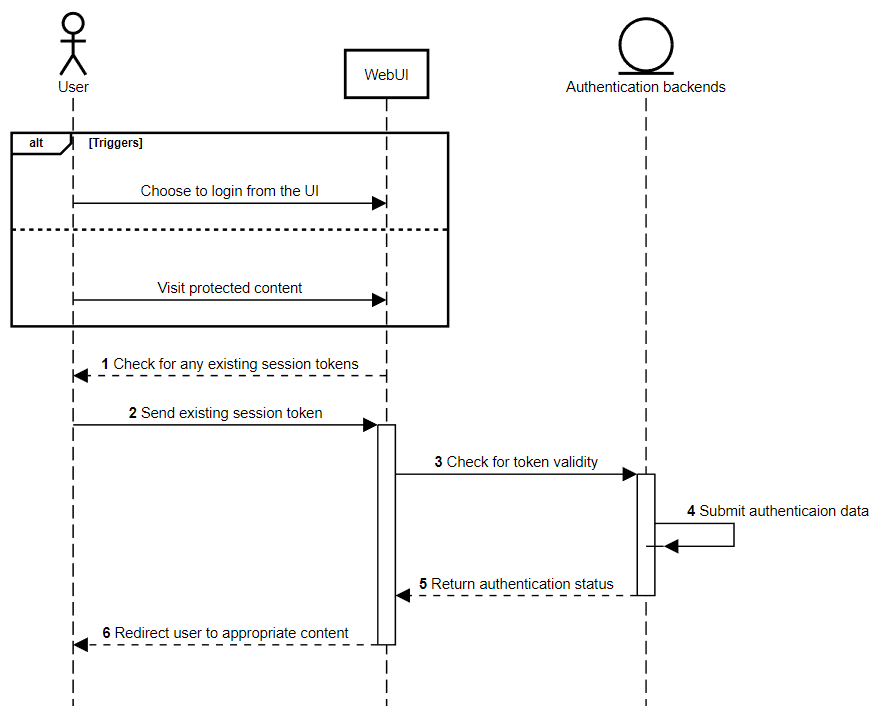
\includegraphics[width=1.0\textwidth]{login (alternative).png}
        \caption{Sequence diagram for the login use case (alternative flow)}
        \label{fig:fig8}
    \end{figure}

    \begin{figure}[H]
        \centering
        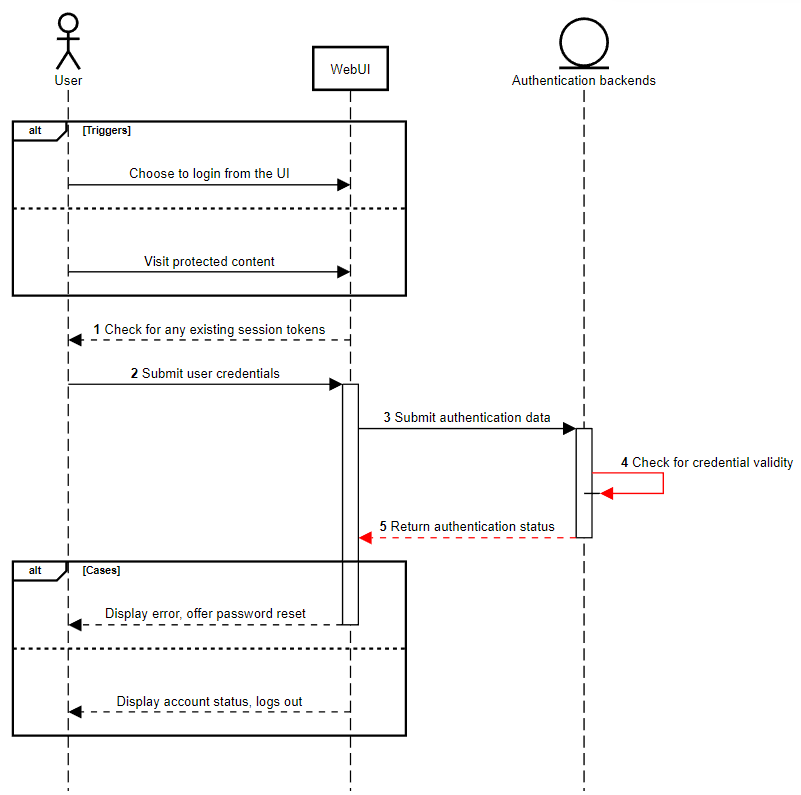
\includegraphics[width=1.0\textwidth]{login (exception).png}
        \caption{Sequence diagram for the login use case (exception flow)}
        \label{fig:fig9}
    \end{figure}

    \begin{figure}[H]
        \centering
        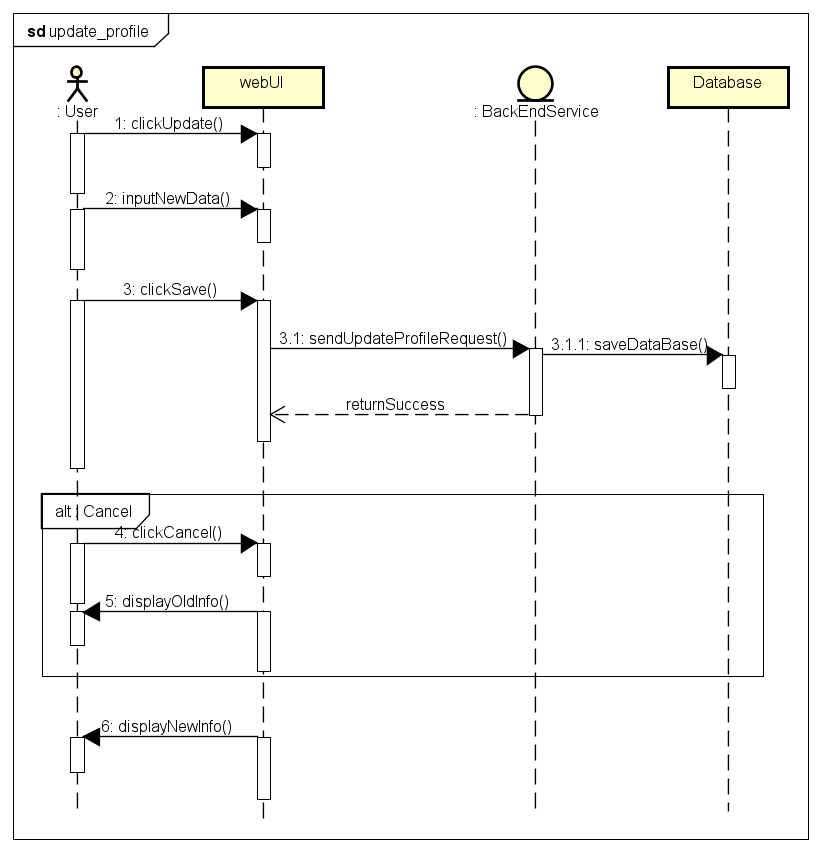
\includegraphics[width=1.0\textwidth]{update_profile.png}
        \caption{Sequence diagram for the update profile use case}
        \label{fig:fig10}
    \end{figure}

    \begin{figure}[H]
        \centering
        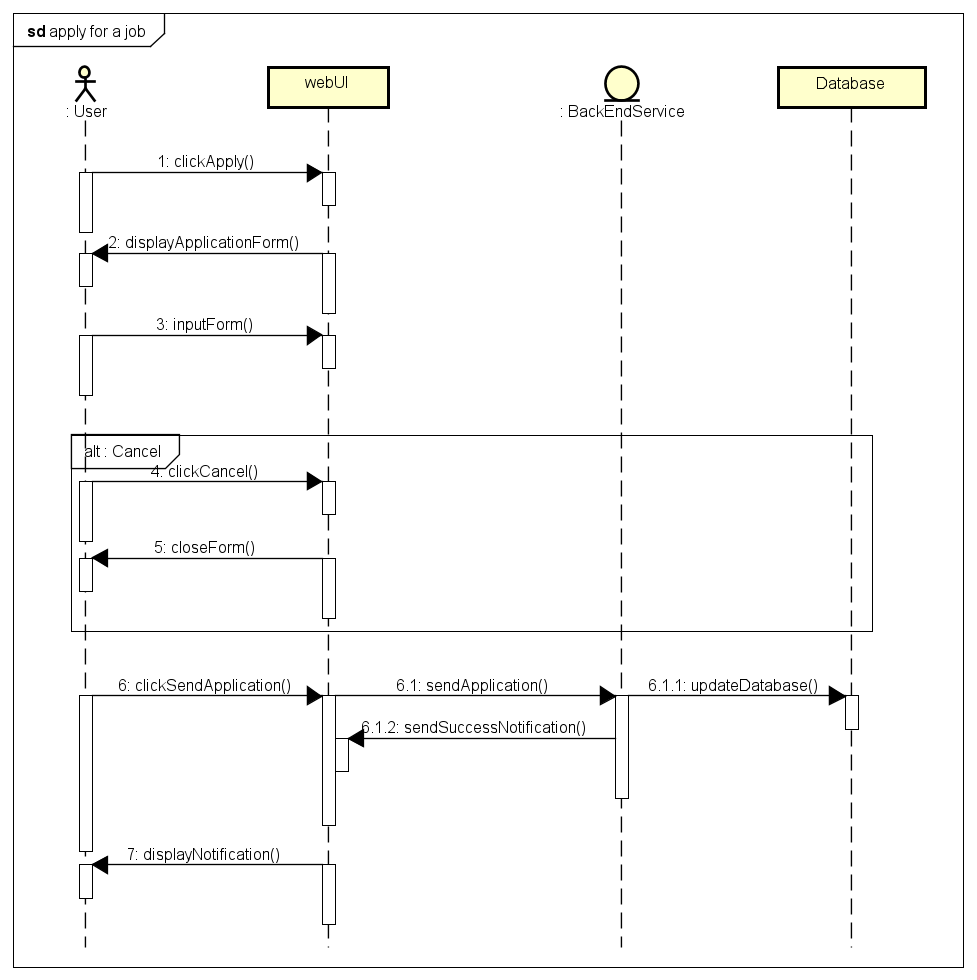
\includegraphics[width=1.0\textwidth]{apply for a job.png}
        \caption{Sequence diagram for the job description application use case}
        \label{fig:fig11}
    \end{figure}

    \begin{figure}[H]
        \centering
        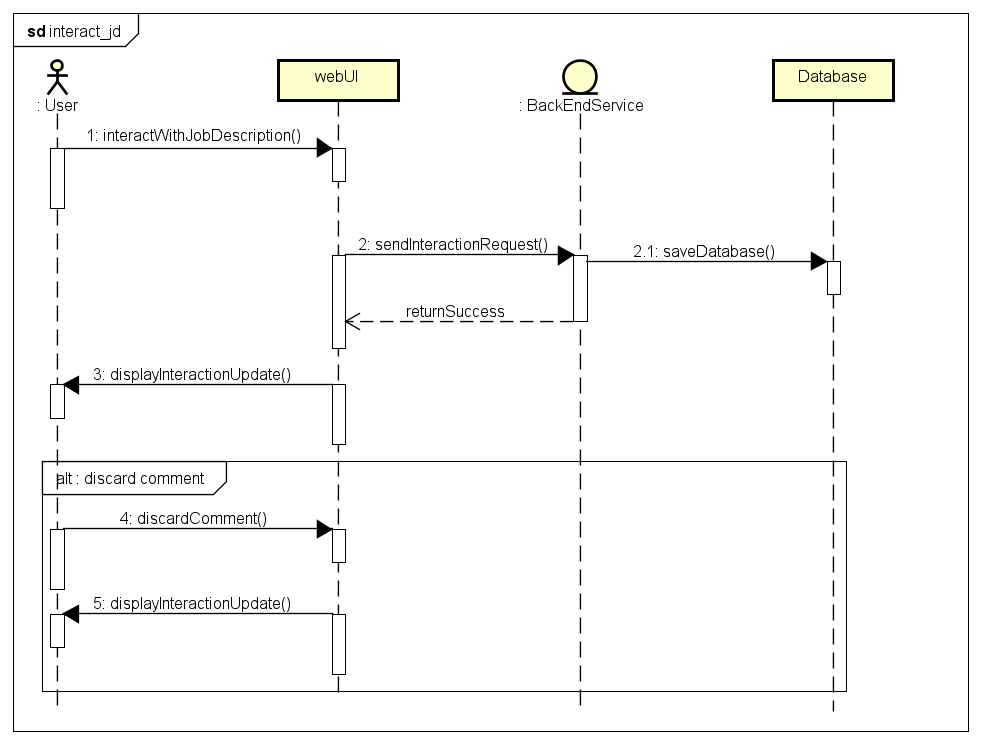
\includegraphics[width=1.0\textwidth]{interact_jd.png}
        \caption{Sequence diagram for the job description interaction use case}
        \label{fig:fig12}
    \end{figure}

    \begin{figure}[H]
        \centering
        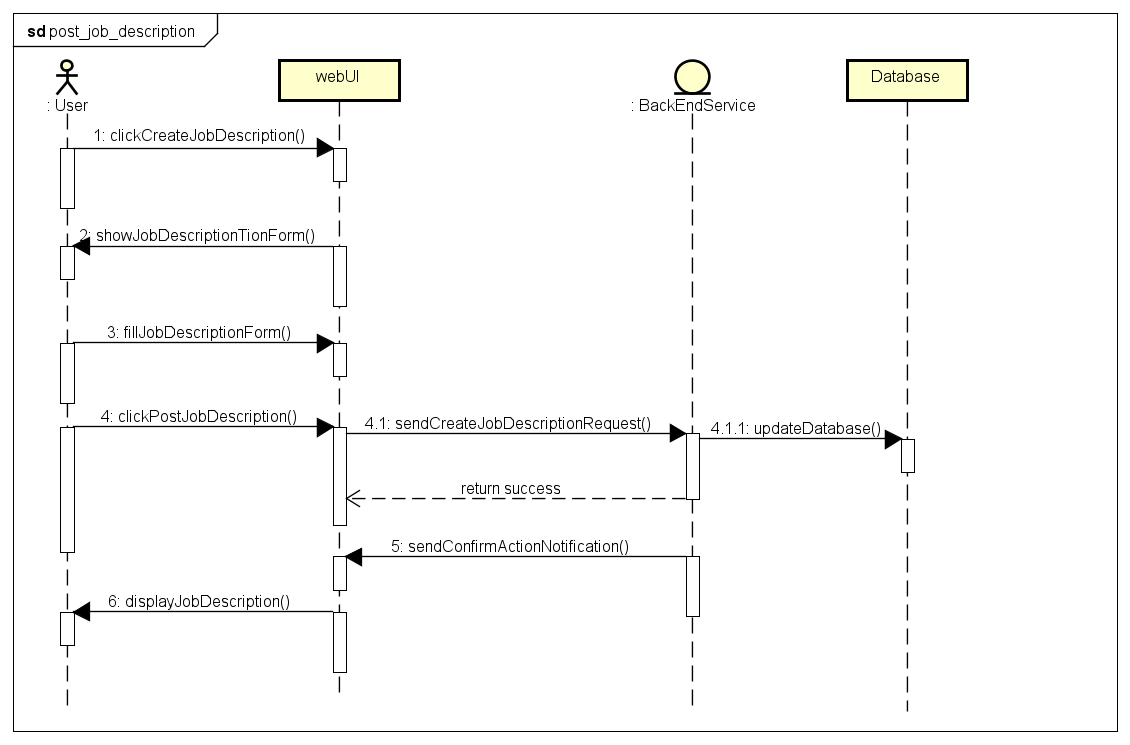
\includegraphics[width=1.0\textwidth]{post_job_description.png}
        \caption{Sequence diagram for the post job description use case}
        \label{fig:fig13}
    \end{figure}

    \begin{figure}[H]
        \centering
        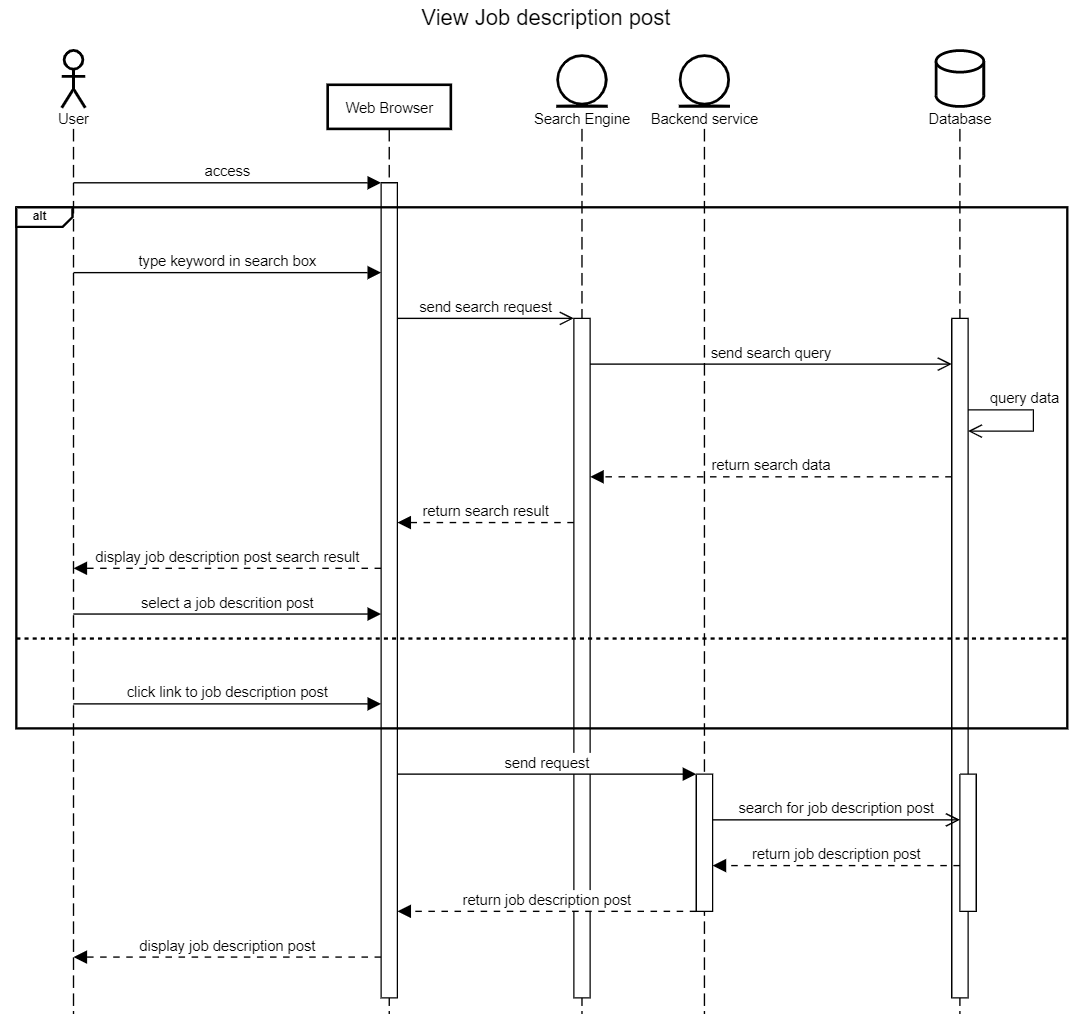
\includegraphics[width=1.0\textwidth]{View job description .png}
        \caption{Sequence diagram for the view job description use case}
        \label{fig:fig14}
    \end{figure}

    \begin{figure}[H]
        \centering
        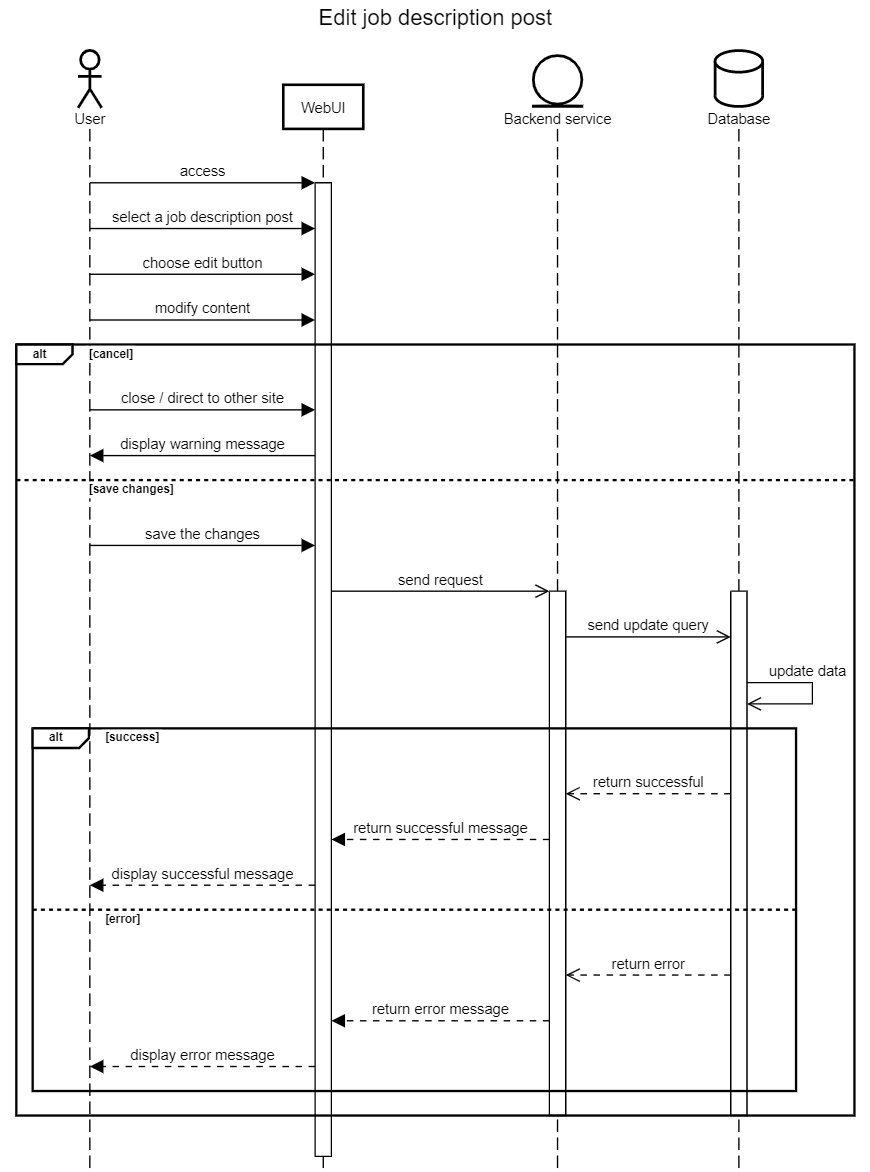
\includegraphics[width=1.0\textwidth]{Edit job description post.png}
        \caption{Sequence diagram for the view job description use case}
        \label{fig:fig15}
    \end{figure}

    \begin{figure}[H]
        \centering
        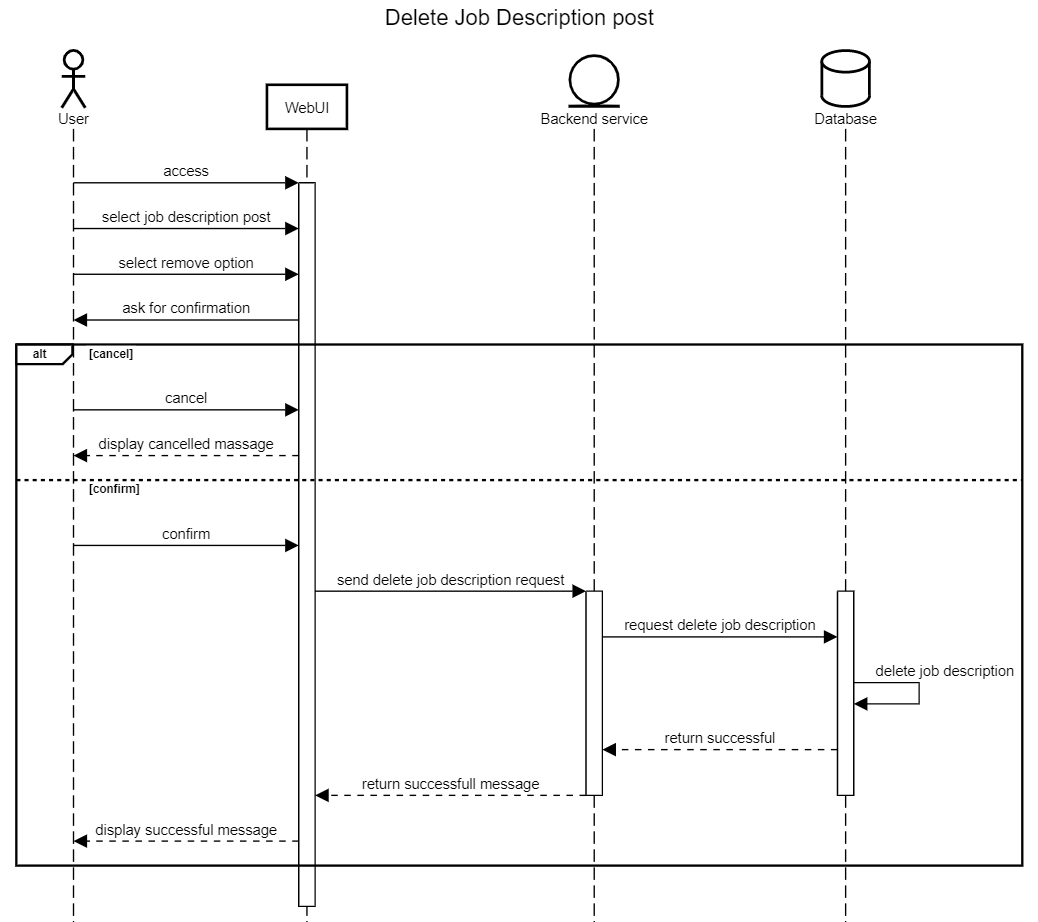
\includegraphics[width=1.0\textwidth]{Delete job description post.png}
        \caption{Sequence diagram for the delete job description use case}
        \label{fig:fig16}
    \end{figure}

    \begin{figure}[H]
        \centering
        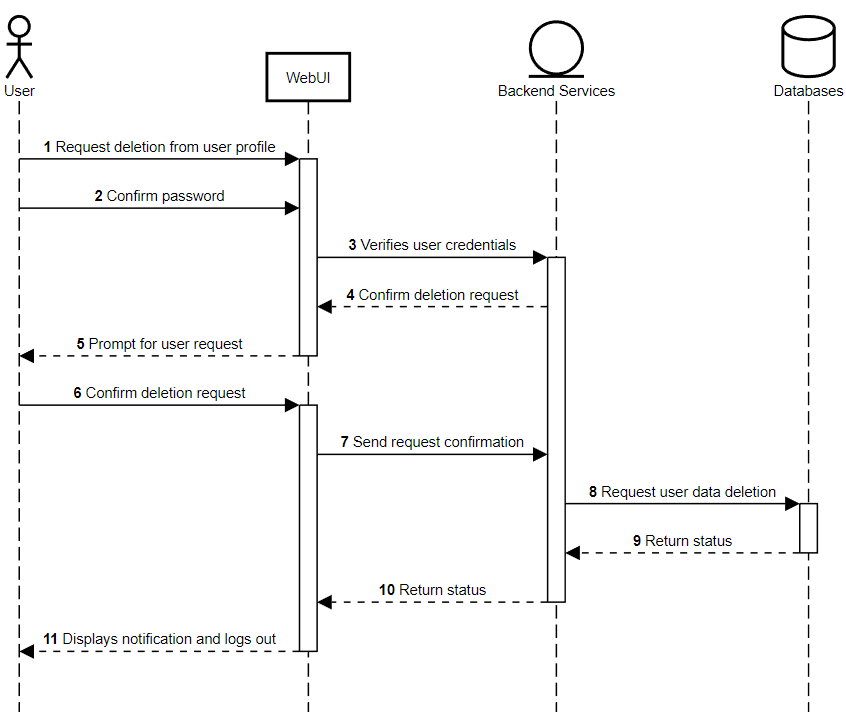
\includegraphics[width=1.0\textwidth]{delete_account.png}
        \caption{Sequence diagram for the delete account use case (basic flow)}
        \label{fig:fig17}
    \end{figure}

    \begin{figure}[H]
        \centering
        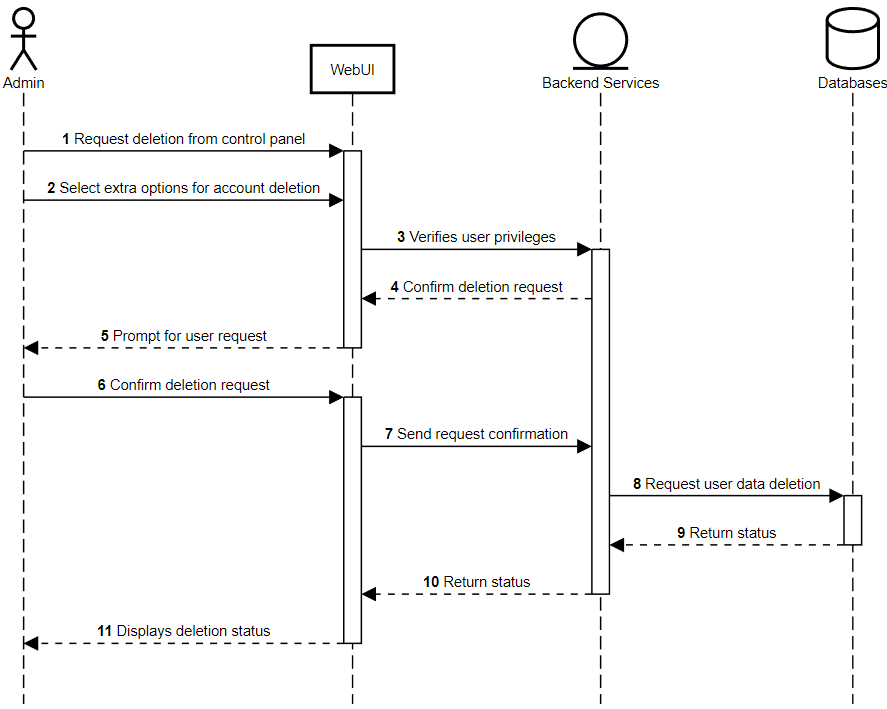
\includegraphics[width=1.0\textwidth]{delete_account (admin).png}
        \caption{Sequence diagram for the post job description use case (admin alternative)}
        \label{fig:fig18}
    \end{figure}

    \begin{figure}[H]
        \centering
        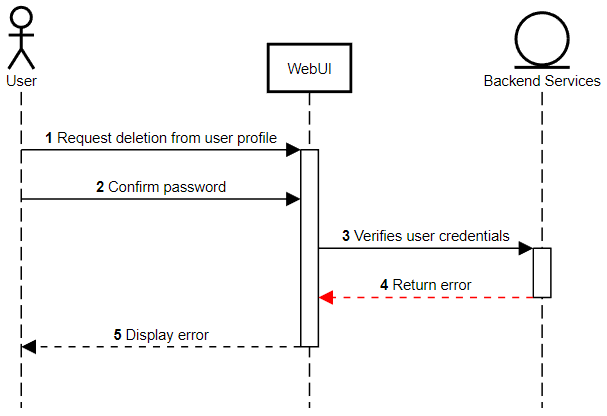
\includegraphics[width=1.0\textwidth]{delete_account (exception).png}
        \caption{Sequence diagram for the delete account use case (exception)}
        \label{fig:fig19}
    \end{figure}

    \begin{figure}[H]
        \centering
        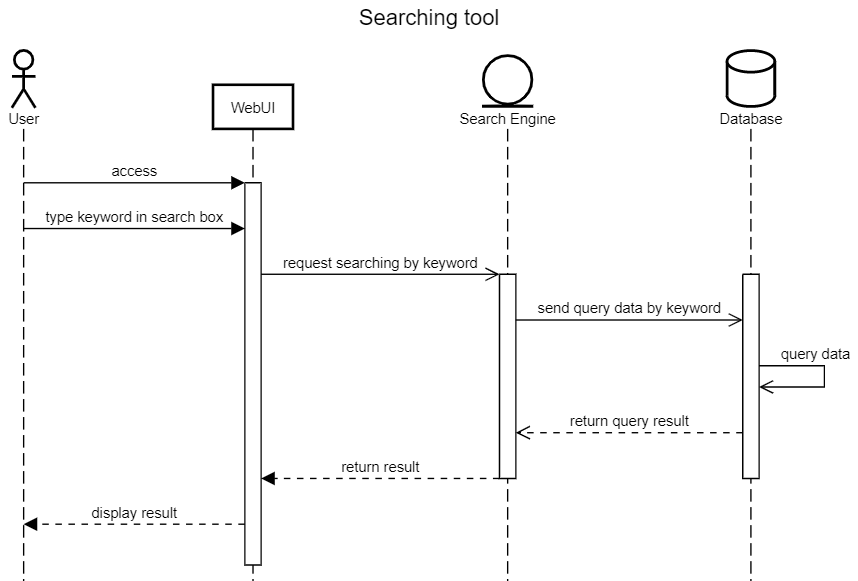
\includegraphics[width=1.0\textwidth]{Searching tool.png}
        \caption{Sequence diagram for the search engine use case}
        \label{fig:fig20}
    \end{figure}

    \subsection{Views of participating classes}
    \begin{figure}[H]
        \centering
        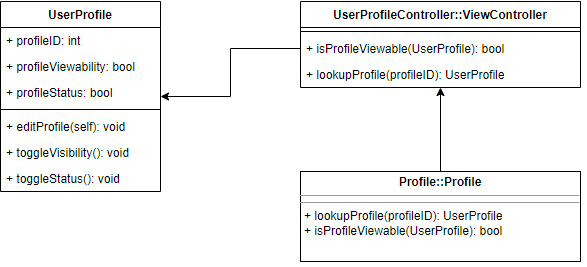
\includegraphics[width=1.0\textwidth]{vopc_view_profile.png}
        \caption{Vopc of view profile use case}
        \label{fig:fig21}
    \end{figure}

    \begin{figure}[H]
        \centering
        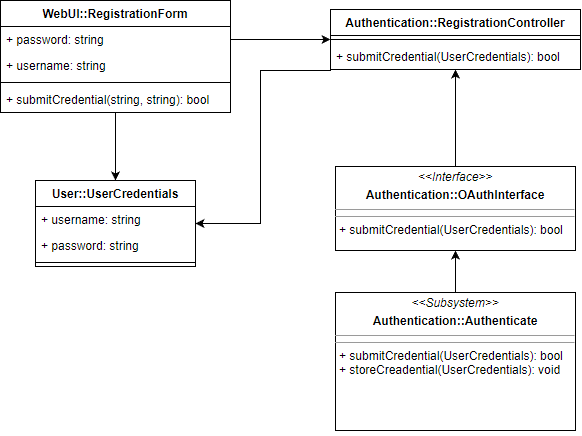
\includegraphics[width=1.0\textwidth]{vopc_register.png}
        \caption{Vopc of create account use case}
        \label{fig:fig22}
    \end{figure}

    \begin{figure}[H]
        \centering
        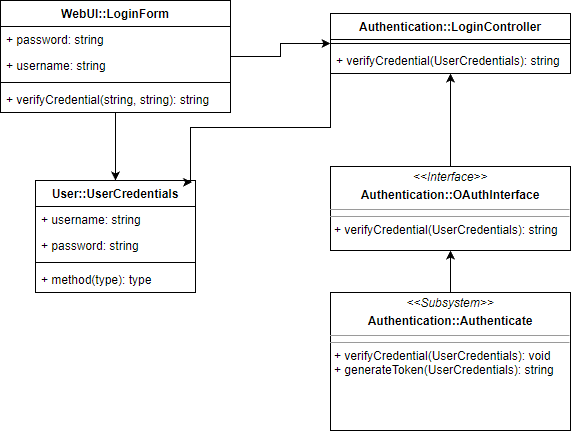
\includegraphics[width=1.0\textwidth]{vopc_login.png}
        \caption{Vopc of login use case}
        \label{fig:fig23}
    \end{figure}

    \begin{figure}[H]
        \centering
        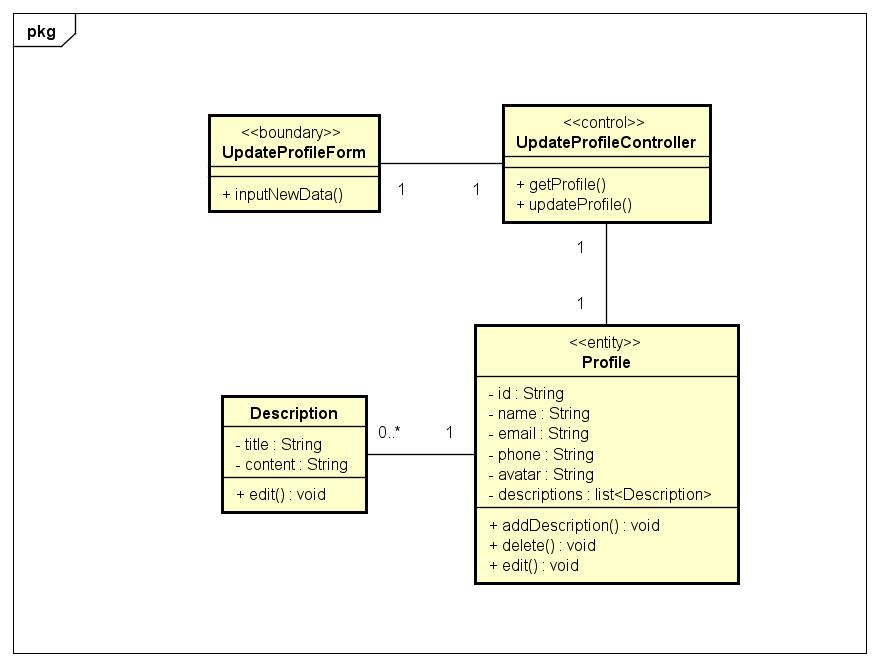
\includegraphics[width=1.0\textwidth]{vopc_update_profile.png}
        \caption{Vopc of update profile use case}
        \label{fig:fig24}
    \end{figure}

    \begin{figure}[H]
        \centering
        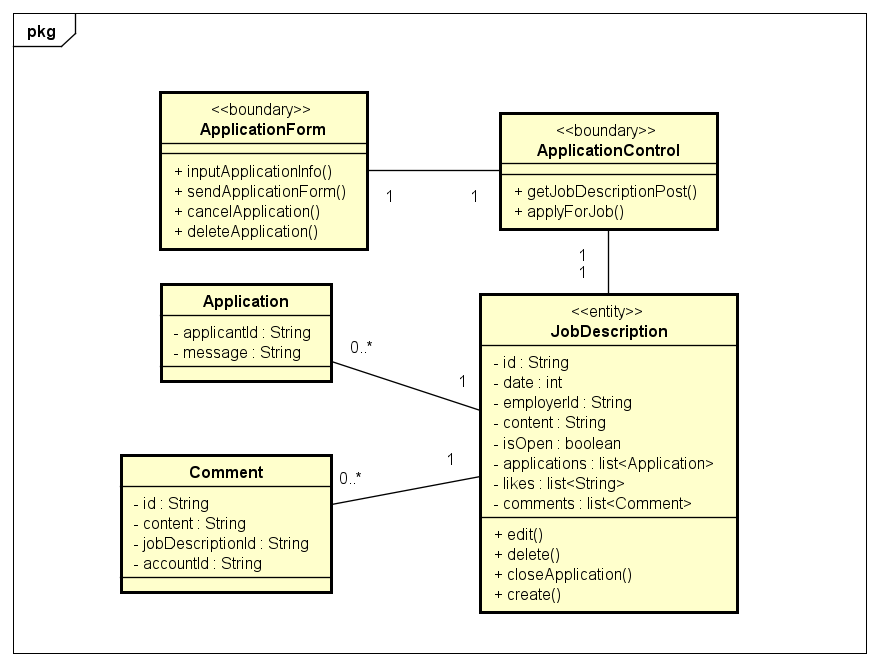
\includegraphics[width=1.0\textwidth]{vopc_job_application.png}
        \caption{Vopc of job application use case}
        \label{fig:fig25}
    \end{figure}

    \begin{figure}[H]
        \centering
        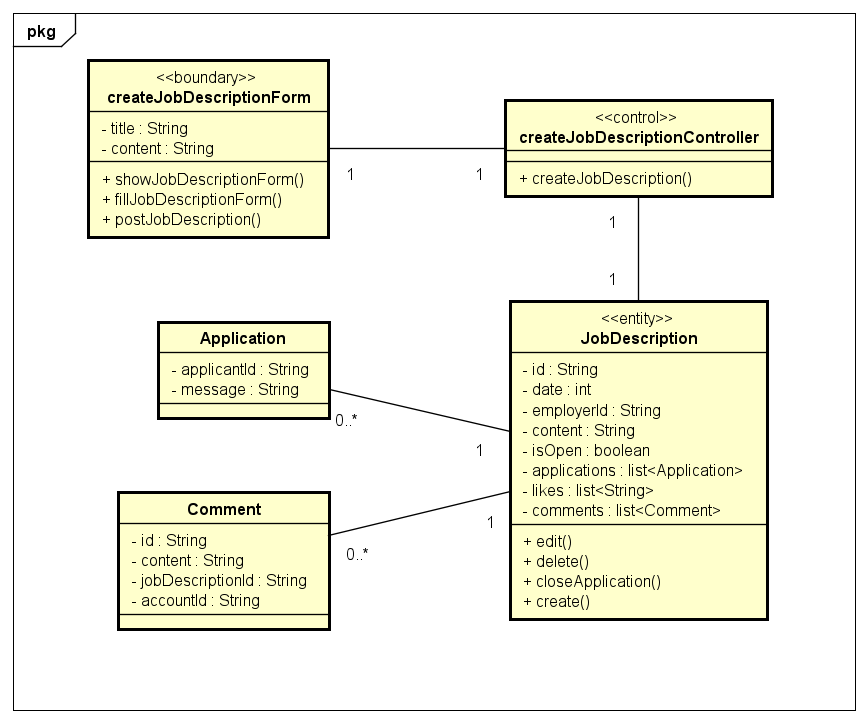
\includegraphics[width=1.0\textwidth]{vopc_post_jd.png}
        \caption{Vopc of post job description use case}
        \label{fig:fig26}
    \end{figure}

    \begin{figure}[H]
        \centering
        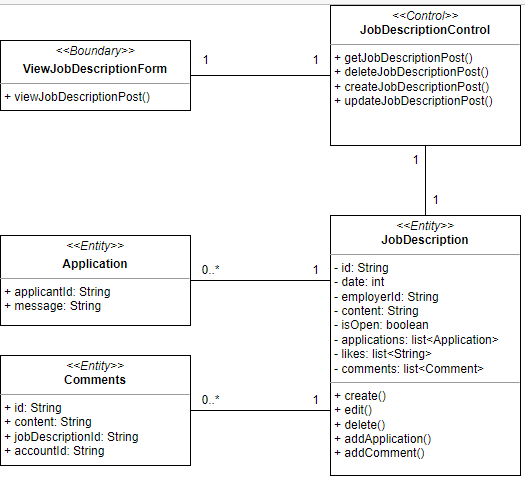
\includegraphics[width=1.0\textwidth]{vopc_view_jd.png}
        \caption{Vopc of view job description use case}
        \label{fig:fig27}
    \end{figure}

    \begin{figure}[H]
        \centering
        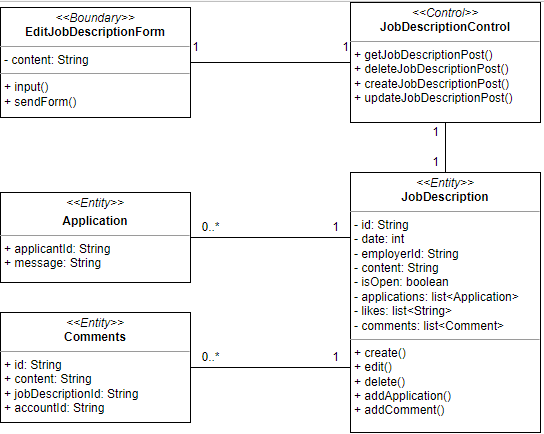
\includegraphics[width=1.0\textwidth]{vopc_edit_jd.png}
        \caption{Vopc of edit job description use case}
        \label{fig:fig28}
    \end{figure}

    \begin{figure}[H]
        \centering
        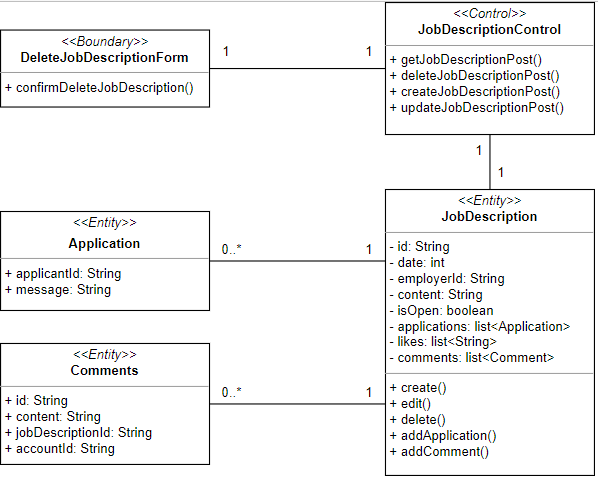
\includegraphics[width=1.0\textwidth]{vopc_del_jd.png}
        \caption{Vopc of delete job description use case}
        \label{fig:fig29}
    \end{figure}

    \begin{figure}[H]
        \centering
        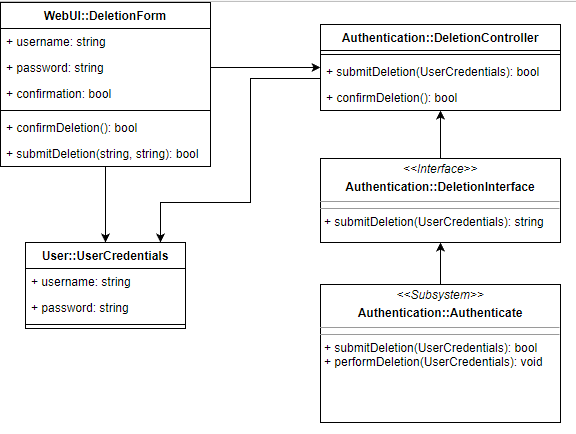
\includegraphics[width=1.0\textwidth]{vopc_delacc.png}
        \caption{Vopc of delete account use case}
        \label{fig:fig30}
    \end{figure}

    \begin{figure}[H]
        \centering
        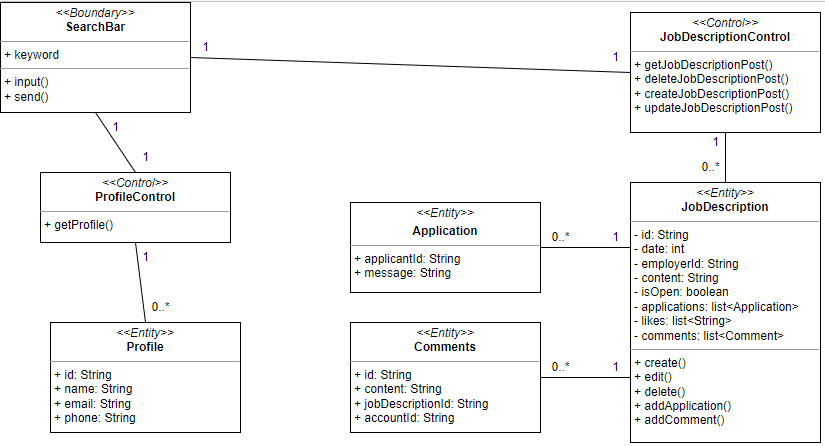
\includegraphics[width=1.0\textwidth]{vopc_search_engine.png}
        \caption{Vopc of search engine use case}
        \label{fig:fig31}
    \end{figure}

\section{Use case design}

    \subsection{Identify classes}
    \begin{center}
        \begin{tabular} { | l | l | }
            \hline
            \textbf{Analysis class} & \textbf{Design element} \\
            \hline
            Account & Account, Database subsystem \\
            \hline
            Job description & Job description, Database subsystem \\
            \hline
            UserProfileController & \multirow{16}{*}{Map directly to design classes} \\
            \cline{1-1}
            RegistrationController & \\
            \cline{1-1}
            LoginController & \\
            \cline{1-1}
            UpdateProfileController & \\
            \cline{1-1}
            JobApplicationController & \\
            \cline{1-1}
            JobDescriptionController & \\
            \cline{1-1}
            DeletionController & \\
            \cline{1-1} & \\
            RegistrationForm & \\
            \cline{1-1}
            LoginForm & \\
            \cline{1-1}
            UpdateProfileForm & \\
            \cline{1-1}
            ApplicationForm & \\
            \cline{1-1}
            CreateJobDescriptionForm & \\
            \cline{1-1}
            EditJobDescriptionForm & \\
            \cline{1-1}
            DeleteJobDescriptionForm & \\
            \cline{1-1}
            DeleteAccountForm & \\
            \cline{1-1}
            SearchBarForm & \\
            \hline
        \end{tabular}
    \end{center}

    \subsection{Identify subsystem and interfaces}
    Giang's job

    \subsection{Identify packages}
    \textbf{The Application package}
    \begin{figure}[H]
        \centering
        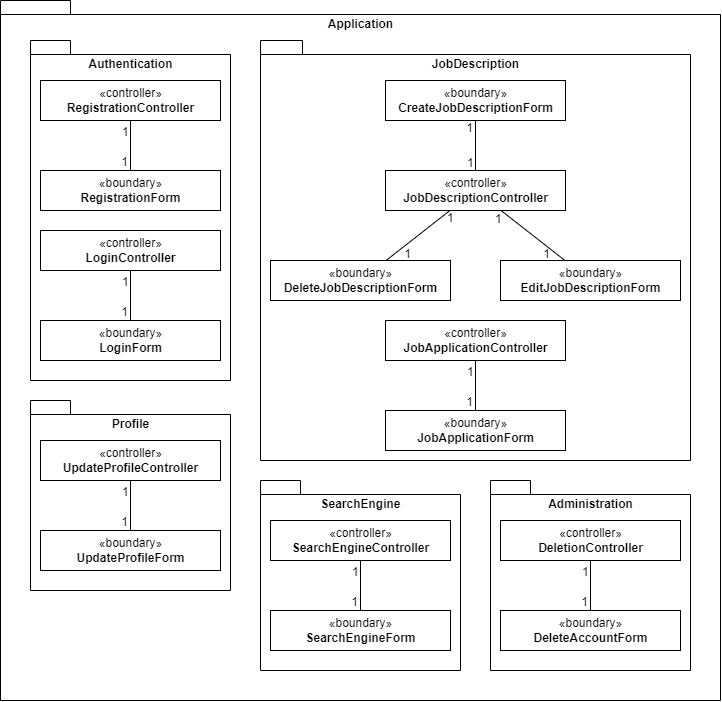
\includegraphics[width=1.0\textwidth]{application_package.drawio.png}
        \caption{Design of the application package}
        \label{fig:fig32}
    \end{figure}

\end{document}
